\documentclass{myassignment}
\usepackage{multicol}

\courselabel{MAT1100}
\exercisesheet{Oblig 1}{Obligatorisk oppgave 1 av 2}

\begin{document}
	\begin{problem}
		Skriv det komplekse tallet $z=\frac{6}{\sqrt{3}+3i}$ først på formen $a+ib$ også på polarformen $re^{i\theta}$.
	\end{problem}

		\begin{multicols}{2}
			\begin{answer}
				\begin{align*}
					z &= \frac{6}{\sqrt{3}+3i} \\[0.4em]
					z &= \frac{2}{\sqrt{\frac{1}{3}}+i} \\[0.4em]
					z &= \frac{2\times(\sqrt{\frac{1}{3}}-i)}{(\sqrt{\frac{1}{3}}+i)\times(\sqrt{\frac{1}{3}}-i)} \\[0.4em]
					z &= \frac{2\times(\sqrt{\frac{1}{3}}-i)}{\frac{1}{3}-i^2} \\[0.4em]
					z &= \frac{2\times(\sqrt{\frac{1}{3}}-i)}{\frac{4}{3}} \\[0.4em]
					z &= \frac{3\times(\sqrt{\frac{1}{3}}-i)}{2} \\[0.4em]
					z &= \frac{\sqrt{3}}{2} - \frac{3}{2}i
				\end{align*}
				\vspace*{\fill}
			\end{answer}

				\vspace*{2em}
				Using $z = \frac{\sqrt{3}}{2} - \frac{3}{2}i$:

				%\raisebox{-.5\height}{
				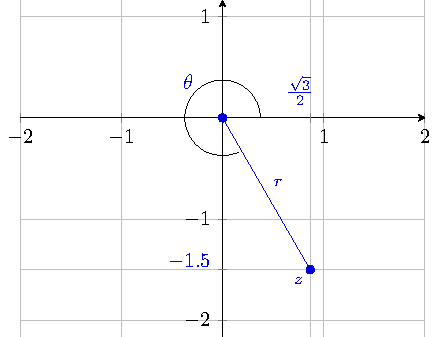
\includegraphics[scale=1]{graphact1.pdf}
				%}
			\columnbreak

			\begin{answer}
				\textit{\hspace*{2em}\small With Pythagora's Theorem}
				\begin{align*}
					r &= \sqrt{(\frac{\sqrt{3}}{2})^2 +(\frac{3}{2})^2}\\
					r &= \sqrt{\frac{3}{4} + \frac{9}{4}} \\
					r &= \sqrt{3}
				\end{align*}
				\blackqed
				\vspace*{-1em}

				\begin{align*}
					\theta' &:= 2\pi - \theta\\[1em]
					\sin(\theta') &= \frac{-1.5}{\sqrt{3}} \\
					\theta' &= \arcsin(\frac{-1.5\sqrt{3}}{3}) \\
					\theta' &= \arcsin(\frac{\sqrt{3}}{2}) \\
					\theta' &= \frac{\pi}{3} \\
					\therefore \theta  &= \frac{5\pi}{3} \\
				\end{align*}
				\blackqed

				\begin{align*}
					r: \sqrt{3} \land \theta: \frac{5\pi}{3} \therefore z = \sqrt{3}e^{i\frac{5\pi}{3}}
				\end{align*}
			\end{answer}
		\end{multicols}
		\pagebreak


	\begin{problem}
		Finn de to løsningene til likningen $w^2 - w + 1 = \theta$, og bruk disse til å finne alle komplekse løsninger til likningen $z^4 - z^2 + 1 = \theta$.Gi en faktorisering av $z^4 - z^2 + 1$, først i komplekse førstegradspolynomer og så i reelle andregradspolynomer.
	\end{problem}

	\begin{answer}

	\end{answer}


	\begin{problem}
		Finn grensene $\lim_{n \rightarrow \infty}\frac{3n + 2}{\sqrt{4n^2 - 1}}$ og $\lim_{n\rightarrow\infty}(\sqrt{n^2 - 5n} - n)$.
	\end{problem}

	\begin{answer}

	\end{answer}


	\begin{problem}
		Finn de komplekse tallenezsom oppfyller likningen $2|z - 1|=|z - 4|$ og skisser løsningsmengden i det komplekse planet.(Hint: Sett inn $z=x+iy$ og finn en polynomlikning ixogyforløsningsmengden.)
	\end{problem}

	\begin{answer}

	\end{answer}


	\begin{problem}
		En følge $\{ a_n \}$ er definert ved $a_1 = 3, a_n + 1 = 3\sqrt{a_n}$ for $n \geq 1$.Vis at $a_n < 9$ og at $a_n+1 > a_n$ for alle $n$. Forklar hvorfor følgen konvergerer og finn $\lim_{n \rightarrow \infty}{a_n}$
	\end{problem}

	\begin{answer}

	\end{answer}.
\end{document}